\section{Bối cảnh khảo sát và mô hình nghiệp vụ}
\subsection{Quy trình tham chiếu và phạm vi dữ liệu}
Phương pháp khảo sát là phân tích quy trình nghiệp vụ tham chiếu của nhóm \cite{quytrinh2026}, từ đó xác định tác nhân, trường hợp sử dụng, trạng thái và quyền thao tác. Dữ liệu phòng do nhóm xây dựng để mô hình hóa tình huống; đây là khảo sát quy trình và phân tích yêu cầu, không phải nghiên cứu thống kê người dùng.

Hai vai trò tài khoản là \code{user} và \code{admin}; OneIoT là hệ thống khóa bên ngoài. Dữ liệu tám tầng/bảy phòng mỗi tầng phục vụ kiểm tra giao diện và lọc phòng.

\subsection{Phương thức tiếp cận phòng trong bản triển khai}
Mỗi phòng có một loại khóa \code{PHYSICAL_KEY} hoặc \code{PIN_CODE} (Bảng~\ref{tab:access-modes}); người đặt không tự đổi phương thức khóa cho một lượt.
{\tabletext\renewcommand{\arraystretch}{1.04}\begin{longtable}{>{\raggedright\arraybackslash}p{\dimexpr0.24\textwidth-2\tabcolsep\relax}>{\raggedright\arraybackslash}p{\dimexpr0.43\textwidth-2\tabcolsep\relax}>{\raggedright\arraybackslash}p{\dimexpr0.33\textwidth-2\tabcolsep\relax}}
\caption{Hai phương thức tiếp cận được model hỗ trợ}\label{tab:access-modes}\\
\toprule \textbf{Loại khóa} & \textbf{Luồng sau khi duyệt} & \textbf{Đặc điểm vận hành}\\\midrule
\endfirsthead
\multicolumn{3}{l}{Hai phương thức tiếp cận (tiếp)}\\
\toprule \textbf{Loại khóa} & \textbf{Luồng sau khi duyệt} & \textbf{Đặc điểm vận hành}\\\midrule
\endhead
\bottomrule\endlastfoot
Khóa cơ/thẻ & User đề xuất giờ nhận; admin chấp nhận hoặc đề xuất lại; có thể khai báo người nhận hộ. Admin xác nhận có mặt trong giờ sử dụng. & Lịch hẹn và ủy quyền hỗ trợ bàn giao chìa; việc trả chìa được thực hiện theo quy trình quản lý phòng.\\\addlinespace[1.5pt]
Khóa số & Phòng được gắn SmartLock; người có quyền tạo PIN theo booking và thời hạn; mã chờ hoặc được gửi qua OneIoT. & Ứng dụng lưu PIN, gửi lệnh qua OneIoT và tiếp nhận sự kiện sử dụng khóa theo phiên kết nối.\\\addlinespace[1.5pt]
\end{longtable}}

\section{Tác nhân, kịch bản sử dụng và luồng nghiệp vụ}
\subsection{Phạm vi của từng tác nhân}
Hình~\ref{fig:uc-overview} mô tả chức năng chung: user quản lý lượt của mình, admin xử lý yêu cầu/tài nguyên. Repository local hoặc filter/service server tiếp tục kiểm quyền sau UI.
\begin{figure}[!htbp]\centering
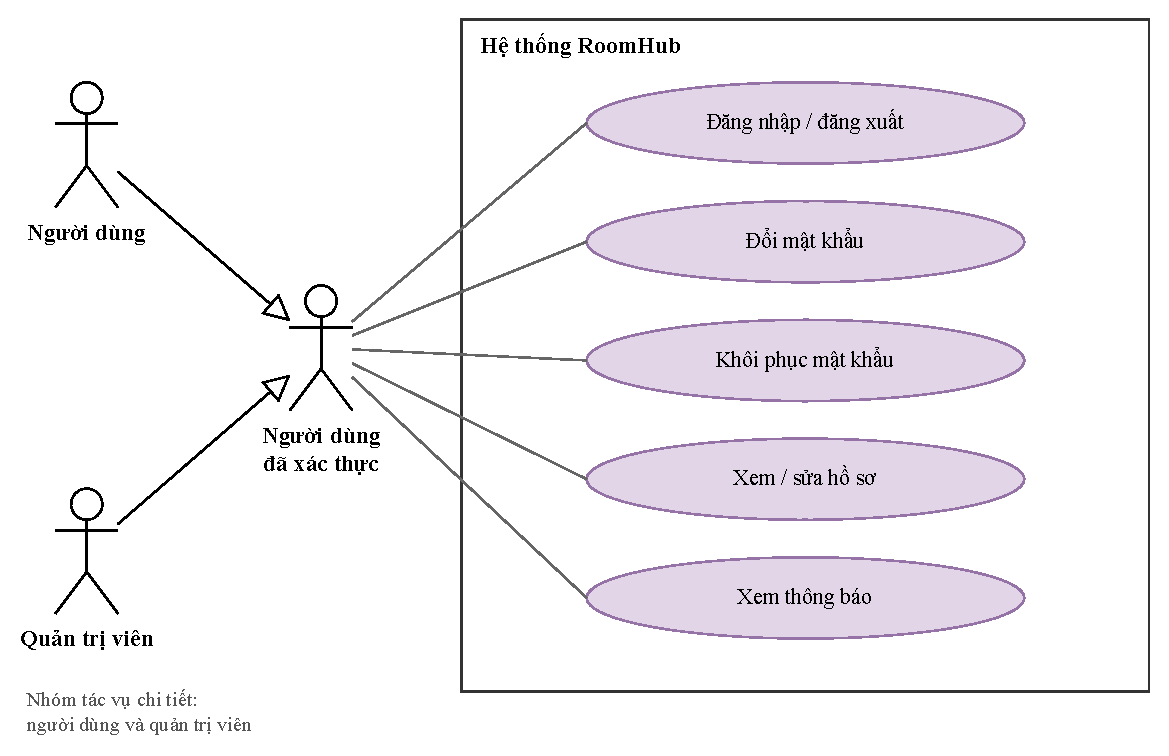
\includegraphics[width=\textwidth,height=.40\textheight,keepaspectratio]{Hinhve/design/02a_use_case_tong_quat.pdf}
\caption{Các use case chung và hai vai trò của RoomHub}\label{fig:uc-overview}
\end{figure}

Hình~\ref{fig:uc-user} tách tác vụ user. Mọi yêu cầu đặt đều được kiểm quy tắc trước nhánh tự duyệt, không do user tự cấp quyền.
\begin{figure}[!htbp]\centering
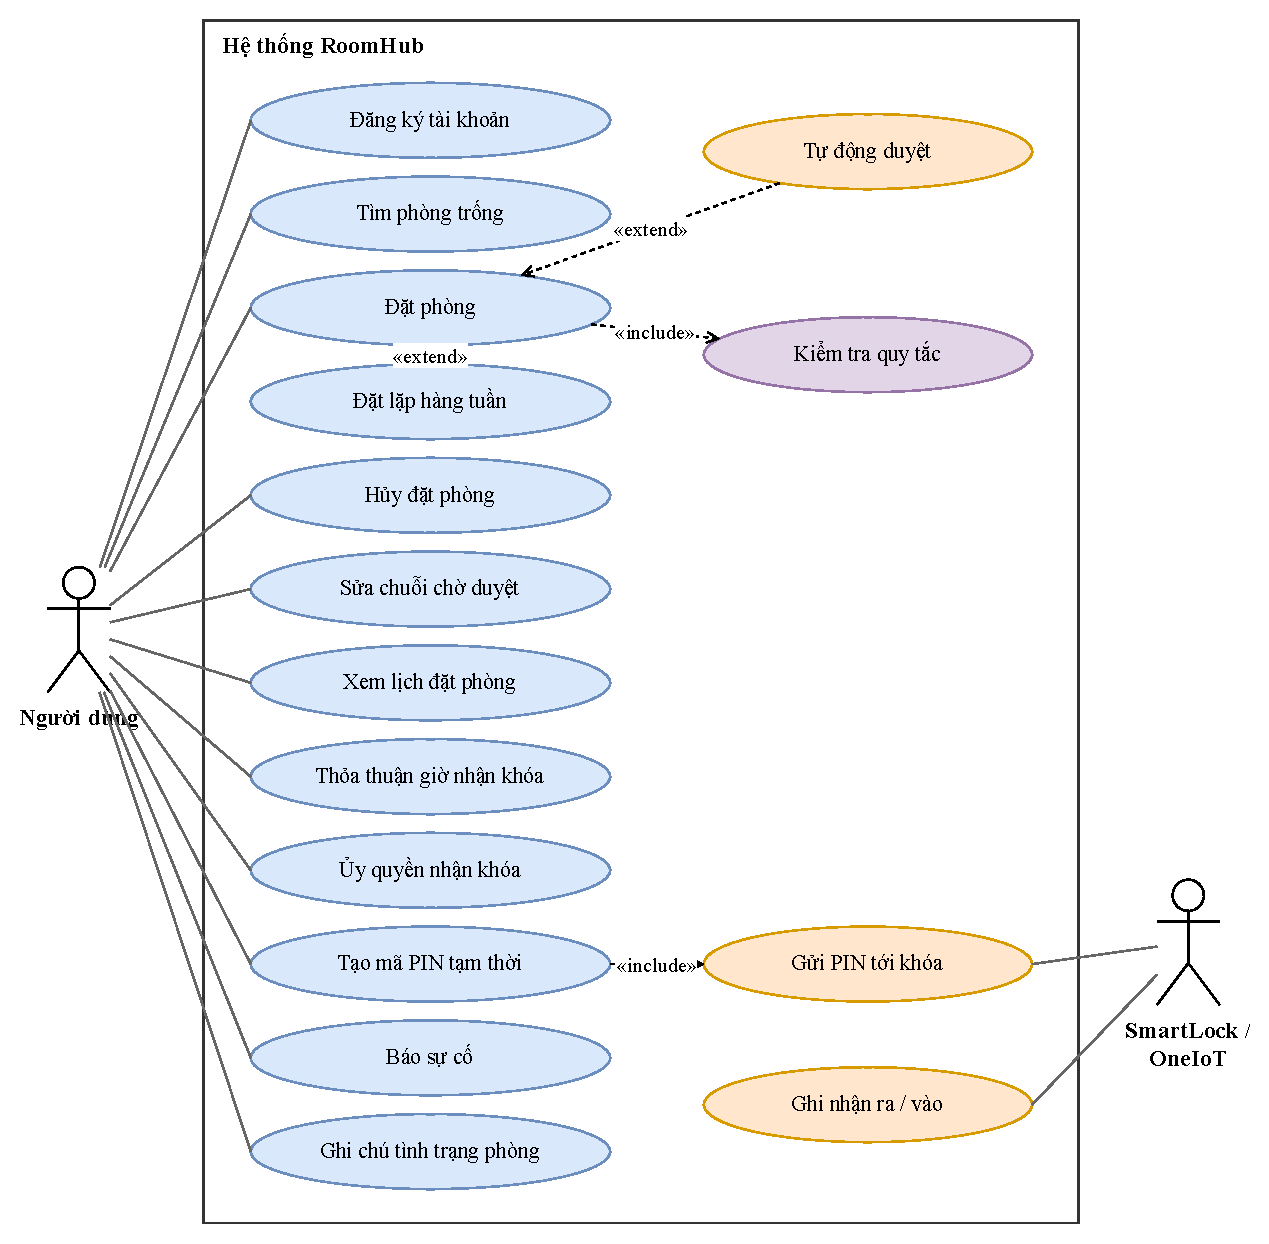
\includegraphics[width=\textwidth,height=.50\textheight,keepaspectratio]{Hinhve/design/02b_use_case_nguoi_dung.pdf}
\caption{Use case của người dùng và tương tác với hệ thống khóa}\label{fig:uc-user}
\end{figure}

Hình~\ref{fig:uc-admin} mô tả tác vụ admin; cấp/thu hồi quyền PIN theo cặp user--phòng không đổi vai trò tài khoản.
\begin{figure}[!htbp]\centering
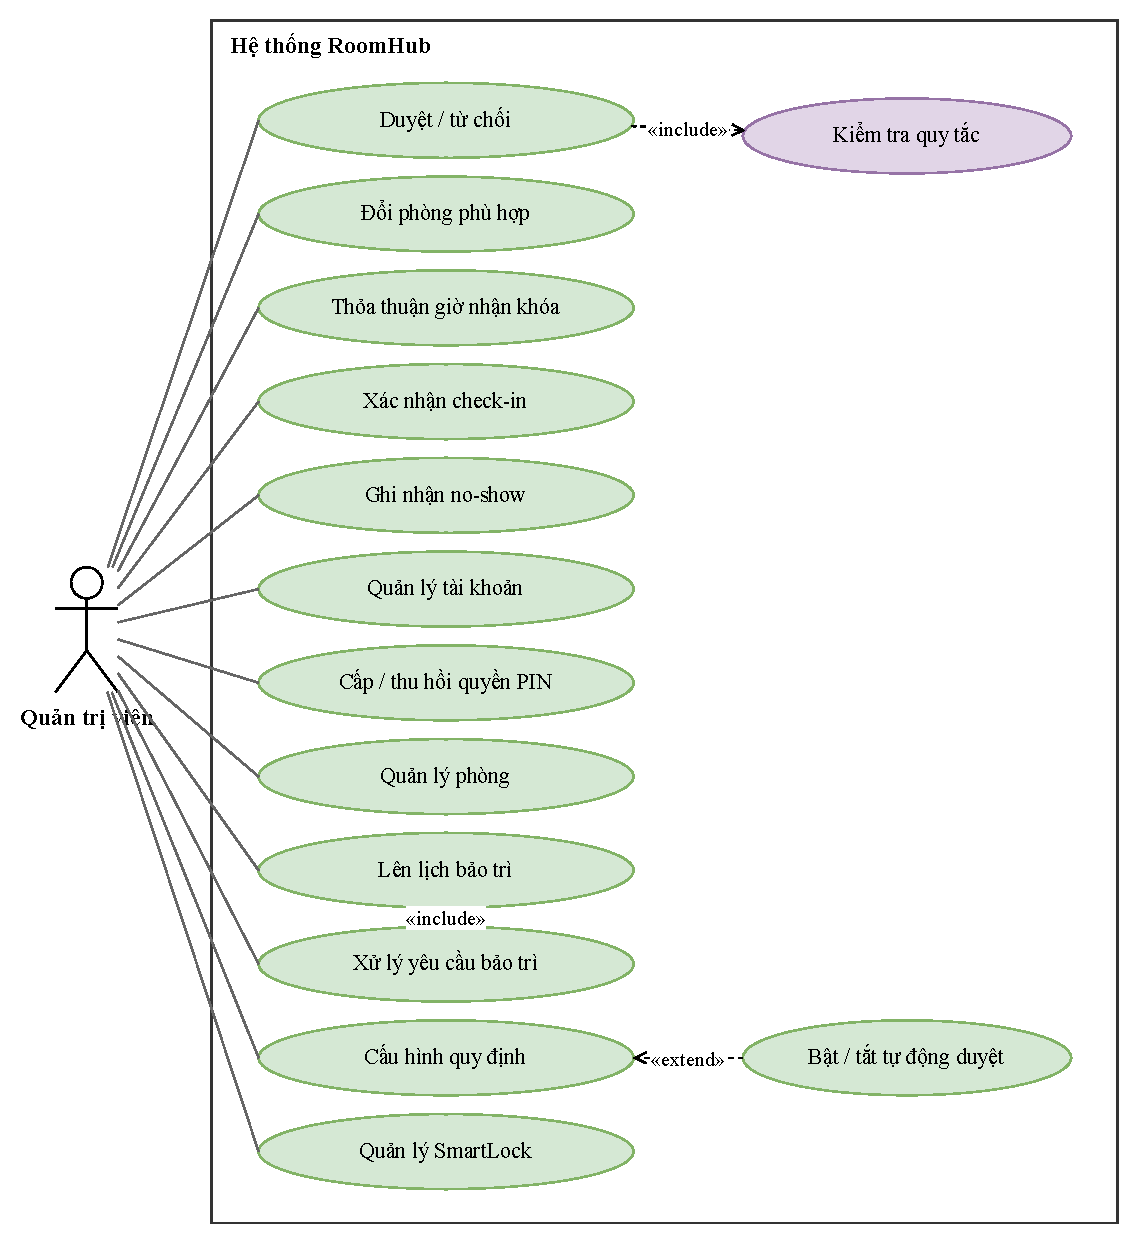
\includegraphics[width=\textwidth,height=.49\textheight,keepaspectratio]{Hinhve/design/02c_use_case_quan_tri_vien.pdf}
\caption{Use case quản trị tài nguyên và xử lý yêu cầu}\label{fig:uc-admin}
\end{figure}
\FloatBarrier

\subsection{Ba kịch bản nghiệp vụ tiêu biểu}
Ba tuyến nghiệp vụ là: đặt/duyệt phòng PIN (UC02, UC03, UC05); nhận chìa, ủy quyền và điểm danh/no-show (UC07, UC12); ghi chú và xử lý bảo trì trong giờ dùng (UC08, UC13). Điều kiện và ngoại lệ được đặc tả tại mục~\ref{sec:use-case-spec}.

\subsection{Đặt phòng, tự duyệt và cấp quyền tiếp cận}
Hình~\ref{fig:activity} thể hiện nhánh REST: UI gửi API, server kiểm điều kiện trước khi quyết định tự duyệt hoặc chuyển admin. Nhánh local thực hiện cùng nhóm quy tắc qua repository thay cho HTTP. Với chuỗi tuần, mọi buổi đều được kiểm xung đột trước khi chốt lưu.
\begin{figure}[H]\centering
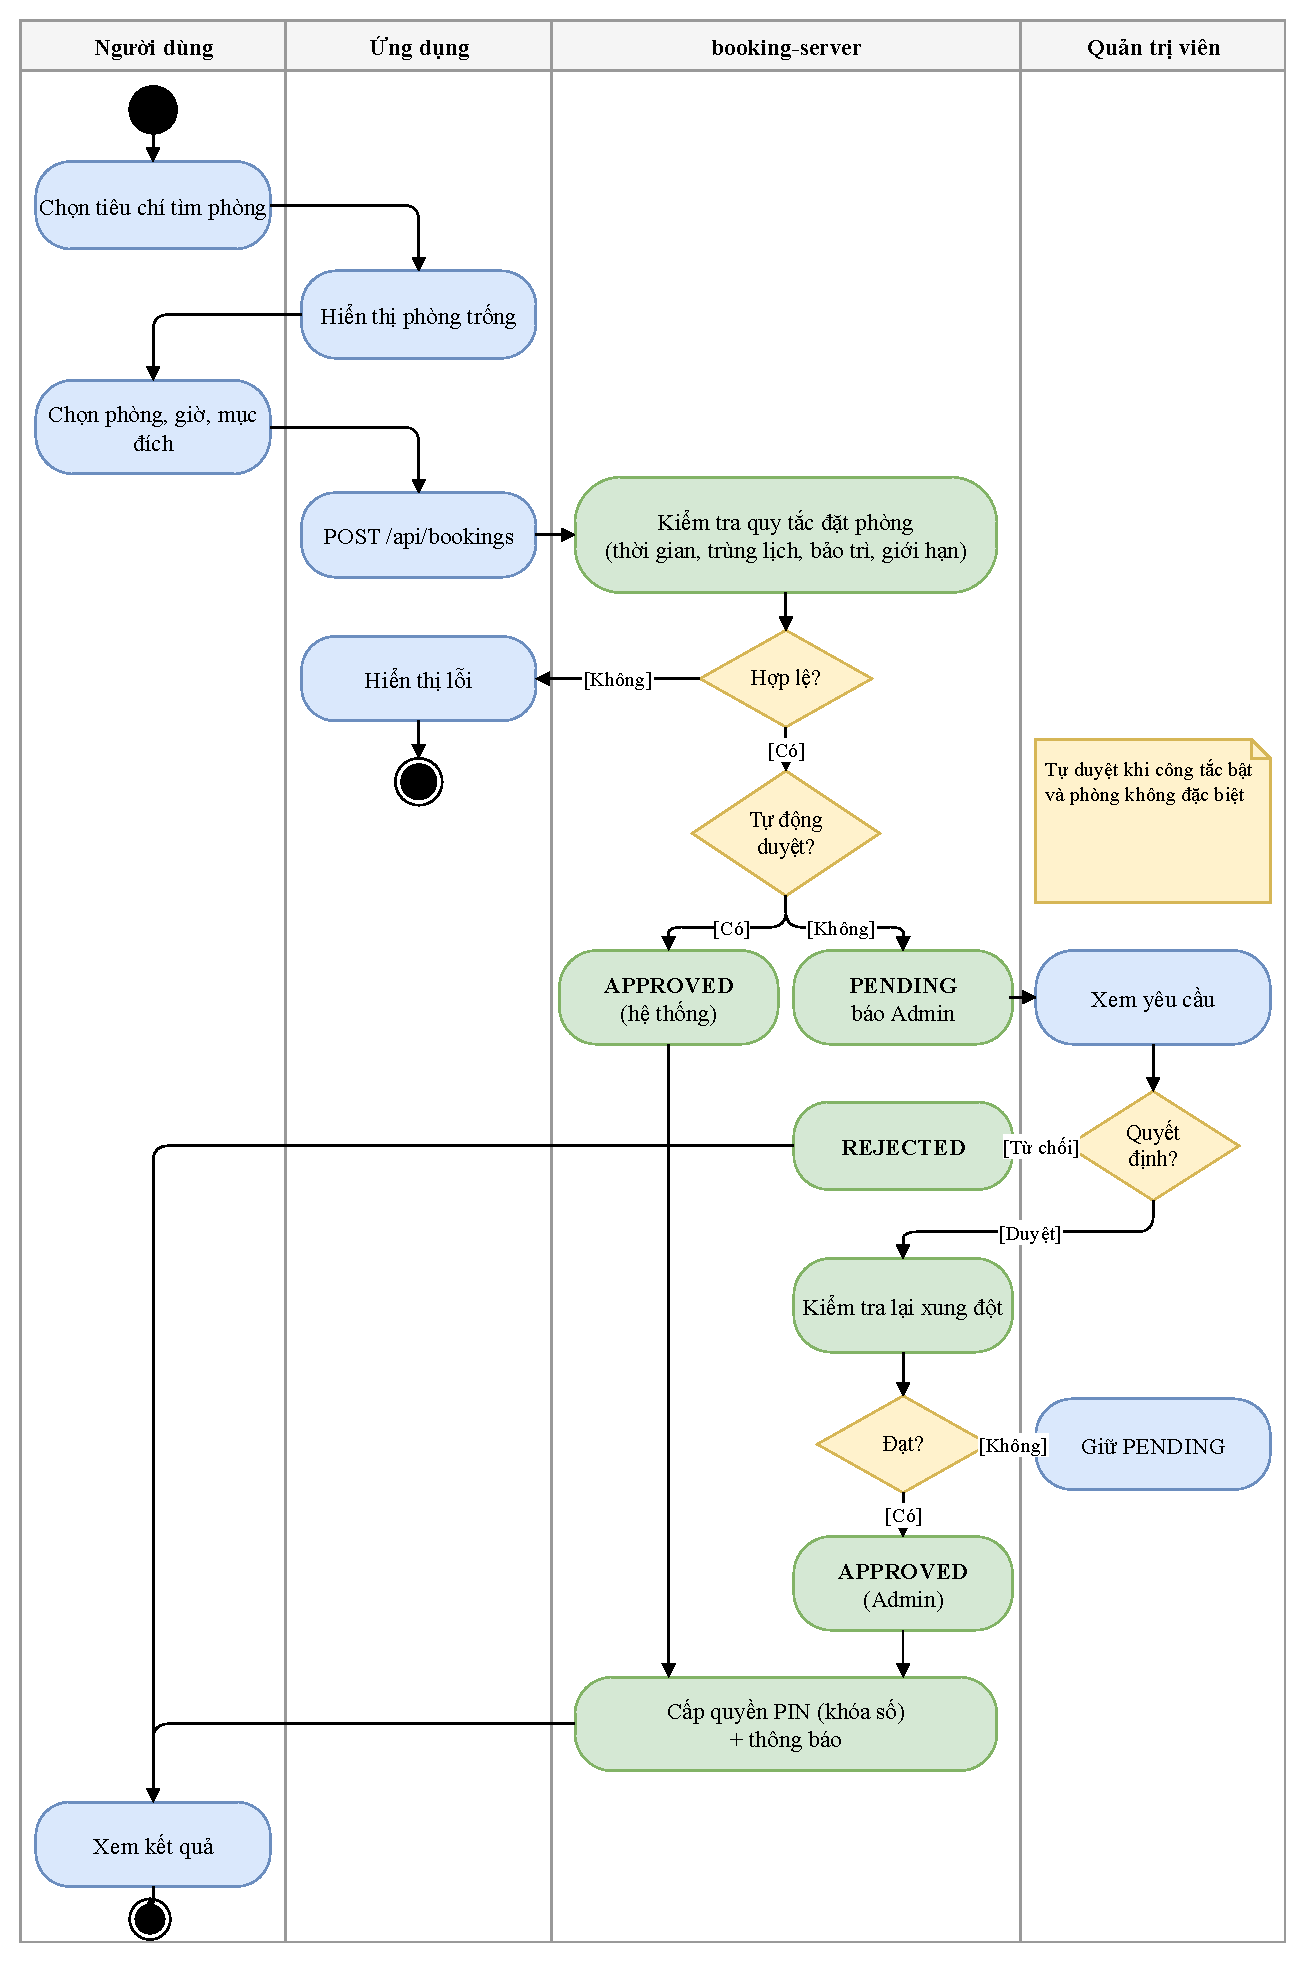
\includegraphics[width=\textwidth,height=.68\textheight,keepaspectratio]{Hinhve/design/03_activity_dat_phong_duyet.pdf}
\caption{Luồng tạo yêu cầu và quyết định duyệt trong nhánh REST}\label{fig:activity}
\end{figure}

Hình~\ref{fig:activity-pin} tách sinh/lưu PIN và gửi lệnh tới khóa. PIN có bảy chữ số; thời hạn lấy từ booking và khoảng đệm cấu hình. Thuộc tính \code{lockDeliveredAt} lưu thời điểm broker nhận lệnh gửi mã. Luồng app--OneIoT--SmartLock đã được nhóm chạy thực tế để sử dụng mã và thao tác khóa.


\begin{figure}[H]\centering
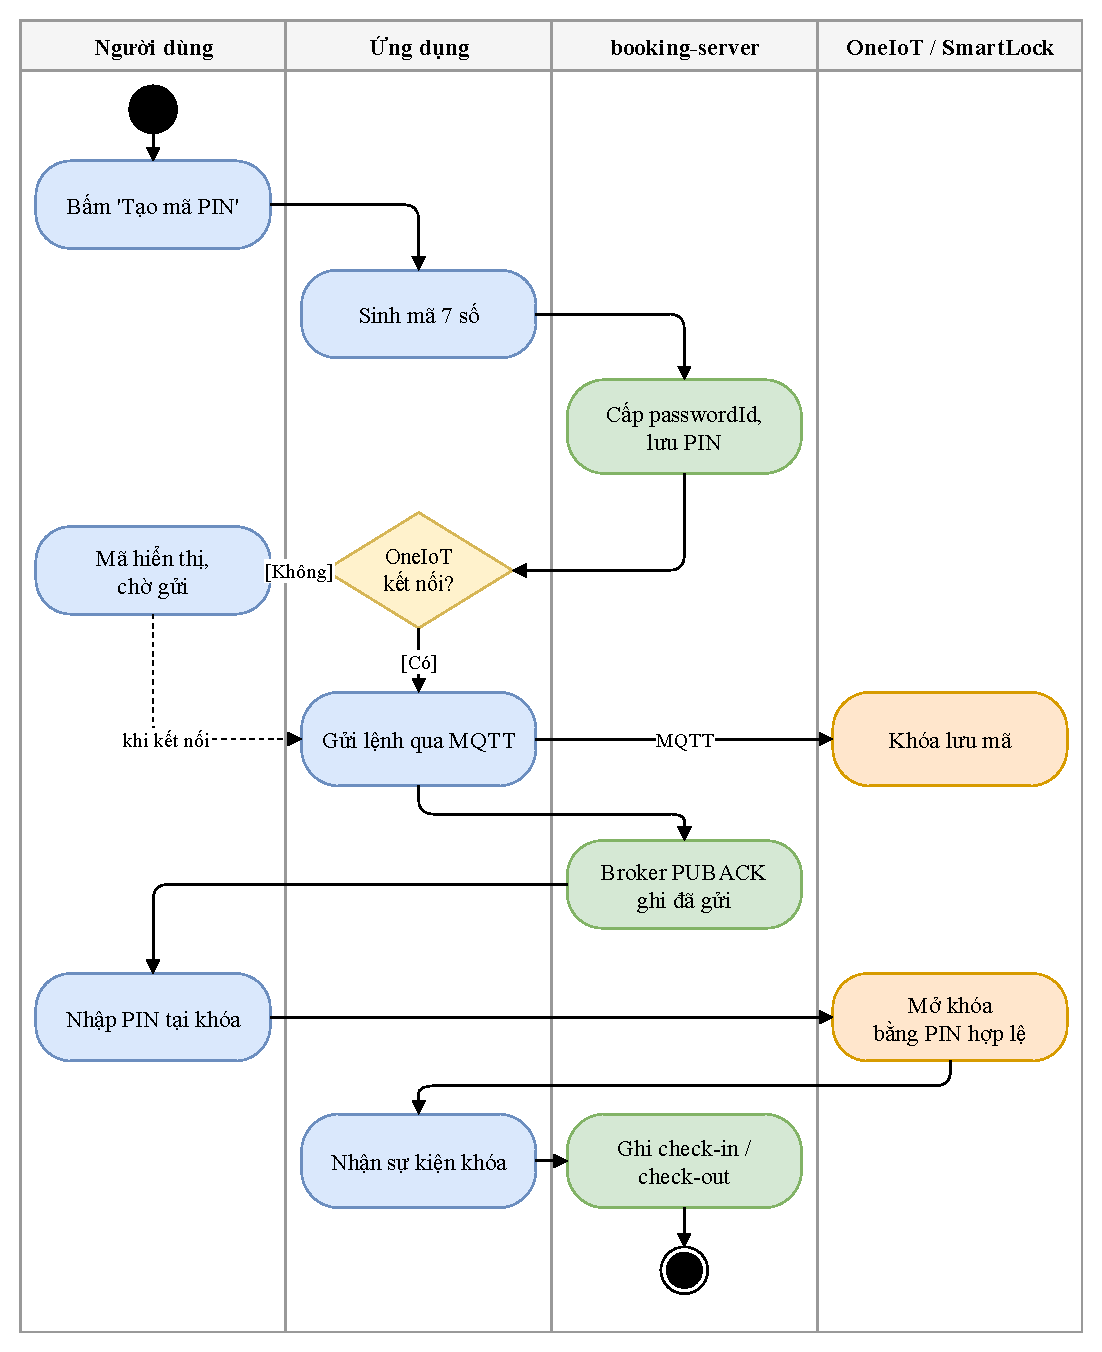
\includegraphics[width=\textwidth,height=.56\textheight,keepaspectratio]{Hinhve/design/04a_activity_khoa_so_pin.pdf}
\caption{Luồng tạo PIN, chờ gửi và giao tiếp OneIoT}\label{fig:activity-pin}
\end{figure}

Hình~\ref{fig:activity-key} giữ riêng lịch nhận khóa, có mặt/vắng mặt và xử lý bảo trì. Lịch hẹn phải ở tương lai và trước giờ sử dụng; check-in thủ công chỉ được ghi trong giờ dùng. Có mặt muộn vẫn có thể được xác nhận nếu booking đang hợp lệ và chưa bị admin đóng bằng no-show.

\begin{figure}[H]\centering
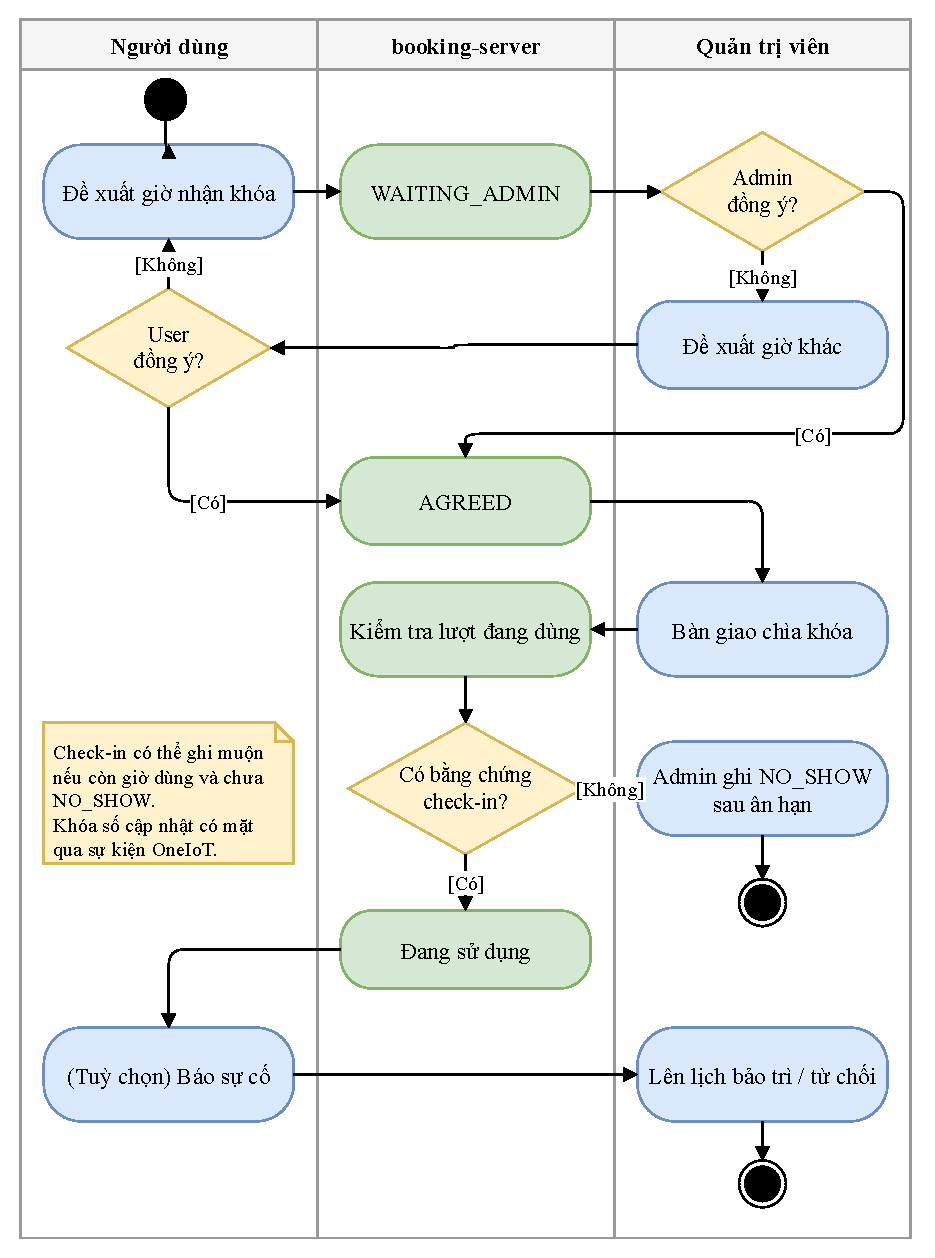
\includegraphics[width=\textwidth,height=.56\textheight,keepaspectratio]{Hinhve/design/04b_activity_khoa_co_vang_mat_bao_tri.pdf}
\caption{Thỏa thuận nhận khóa, xác nhận có mặt và xử lý bảo trì}\label{fig:activity-key}
\end{figure}

\subsection{Vòng đời trạng thái đặt phòng}
Trạng thái lưu là \code{PENDING}, \code{APPROVED}, \code{REJECTED}, \code{CANCELLED} và \code{NO_SHOW}. Tự duyệt cho phép tạo thẳng \code{APPROVED}. Check-in/check-out là các trường/sự kiện bên trong một lượt đã duyệt; đổi phòng không tự đổi trạng thái. Khi hết giờ, UI phân nhóm lượt đã dùng theo thời gian, không ghi thêm trạng thái \code{COMPLETED} vào model. Hình~\ref{fig:booking-state} thể hiện các trạng thái lưu và sự kiện sử dụng của lượt đặt.
\begin{figure}[H]\centering
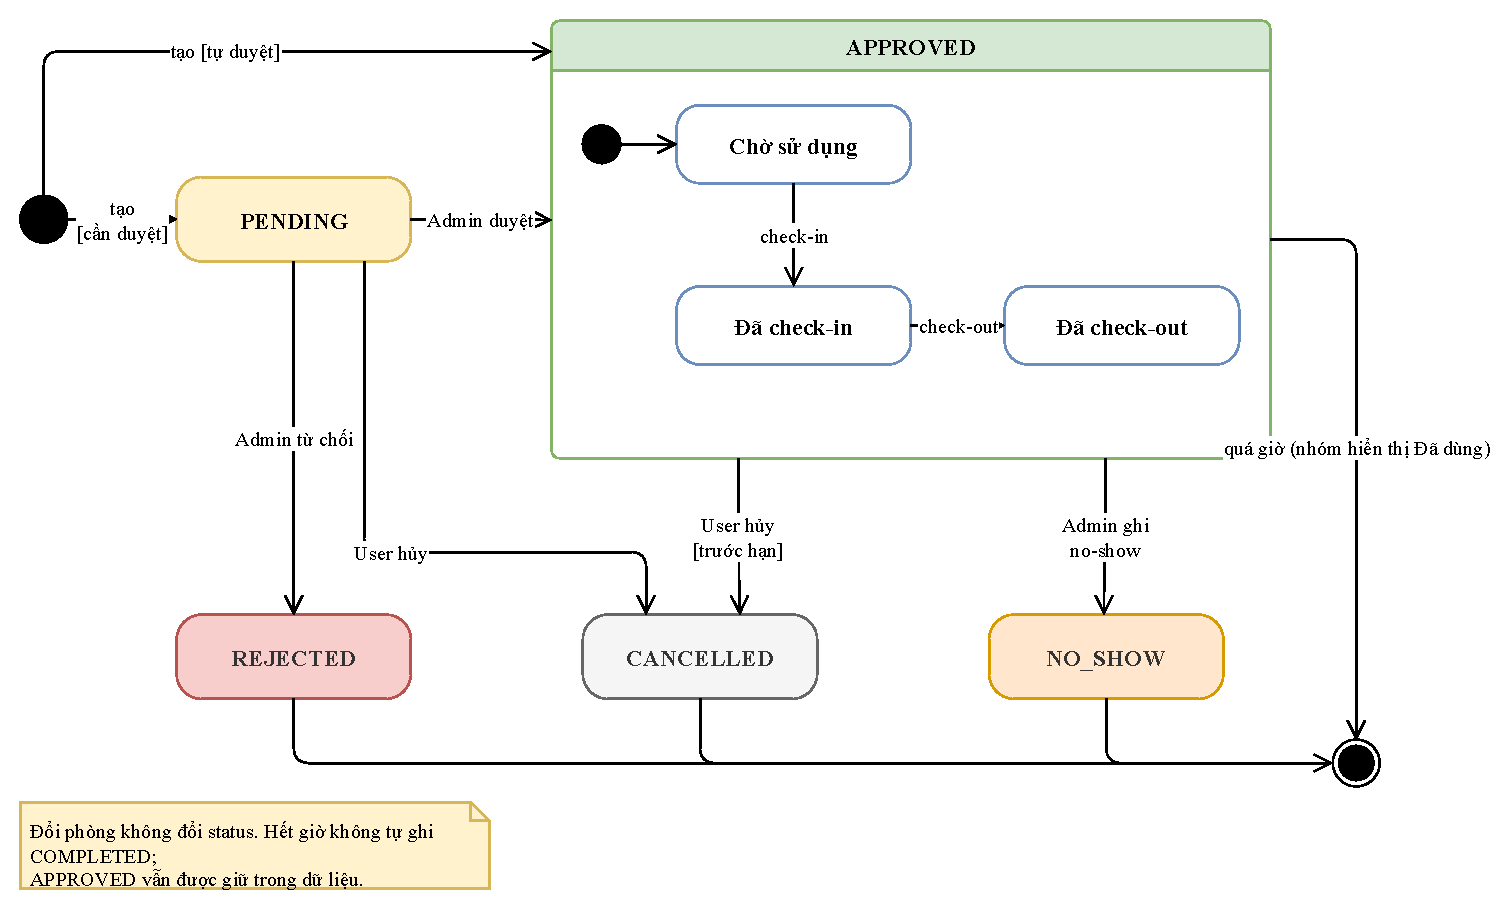
\includegraphics[width=\textwidth,height=.40\textheight,keepaspectratio]{Hinhve/design/18a_state_booking.pdf}
\caption{Vòng đời booking và các mốc sử dụng liên quan}\label{fig:booking-state}
\end{figure}
\FloatBarrier

\section{Yêu cầu chức năng}
{\tabletext\renewcommand{\arraystretch}{1.04}\begin{longtable}{>{\raggedright\arraybackslash}p{\dimexpr0.14\textwidth-2\tabcolsep\relax}>{\raggedright\arraybackslash}p{\dimexpr0.47\textwidth-2\tabcolsep\relax}>{\raggedright\arraybackslash}p{\dimexpr0.39\textwidth-2\tabcolsep\relax}}
\caption{Yêu cầu chức năng và minh chứng kiểm thử}\label{tab:fr}\\
\toprule \textbf{ID / ưu tiên} & \textbf{Yêu cầu và luồng chính} & \textbf{Minh chứng hiện có}\\\midrule
\endfirsthead
\multicolumn{3}{l}{\small Yêu cầu chức năng và minh chứng kiểm thử (tiếp)}\\
\toprule \textbf{ID / ưu tiên} & \textbf{Yêu cầu và luồng chính} & \textbf{Minh chứng hiện có}\\\midrule
\endhead
\bottomrule\endlastfoot
FR01 / Cao & Đăng ký, đăng nhập, đổi/khôi phục mật khẩu; đọc role từ tài khoản. & Ảnh Hình~\ref{fig:ui-roles}; TC01, TC17 và D01--D03.\\\addlinespace[1.5pt]
FR02 / Cao & Tìm phòng theo tầng, giờ, sức chứa, thiết bị, loại khóa; trạng thái theo lịch. & Ảnh Hình~\ref{fig:ui-booking}; TC02, TC12.\\\addlinespace[1.5pt]
FR03 / Cao & Tạo booking một lần/lặp; chặn trùng lịch và bảo trì; hủy/sửa chuỗi theo điều kiện. & TC02, TC11--TC12, TC21; kiểm thử quy tắc và vòng đời đặt phòng.\\\addlinespace[1.5pt]
FR04 / Cao & Admin duyệt/từ chối/đổi phòng; tự duyệt phòng thường khi bật công tắc. & TC07, TC20, TC24; kiểm thử tự duyệt, duyệt tay và đổi phòng.\\\addlinespace[1.5pt]
FR05 / Cao & Quyền PIN theo user--phòng, PIN 7 số và thời hạn; hẹn nhận chìa/ủy quyền. & TC03, TC10, TC13--TC15, TC19; thử nghiệm app--SmartLock.\\\addlinespace[1.5pt]
FR06 / Trung bình & Ghi nhận sự kiện khóa, check-in thủ công khóa cơ và no-show có điều kiện. & TC10, TC22; kiểm thử sự kiện, check-in và ngưỡng no-show.\\\addlinespace[1.5pt]
FR07 / Cao & Tách ghi chú với yêu cầu bảo trì; admin xử lý lịch/yêu cầu. & Ảnh Hình~\ref{fig:ui-room-maintenance}; TC02, TC23.\\\addlinespace[1.5pt]
FR08 / Cao & Admin quản lý tài khoản/phòng/cấu hình; user sửa hồ sơ và xem thông báo. & Ảnh Hình~\ref{fig:ui-roles}; TC06, TC08--TC09, TC16, TC18.\\\addlinespace[1.5pt]
\end{longtable}}

\section{Quy tắc nghiệp vụ và các trường hợp biên}
Bảng~\ref{tab:br} trình bày các mã BR để đặc tả và kiểm thử tham chiếu cùng một quy tắc. Giá trị trong bảng là mặc định của model cấu hình, không phải hằng số cố định cho mọi lần sử dụng.
{\tabletext\renewcommand{\arraystretch}{1.04}\begin{longtable}{>{\raggedright\arraybackslash}p{\dimexpr0.12\textwidth-2\tabcolsep\relax}>{\raggedright\arraybackslash}p{\dimexpr0.66\textwidth-2\tabcolsep\relax}>{\raggedright\arraybackslash}p{\dimexpr0.22\textwidth-2\tabcolsep\relax}}
\caption{Quy tắc nghiệp vụ đối chiếu với mã nguồn}\label{tab:br}\\
\toprule \textbf{Mã} & \textbf{Điều kiện xử lý} & \textbf{Giá trị / phạm vi}\\\midrule
\endfirsthead
\multicolumn{3}{l}{Quy tắc nghiệp vụ (tiếp)}\\
\toprule \textbf{Mã} & \textbf{Điều kiện xử lý} & \textbf{Giá trị / phạm vi}\\\midrule
\endhead
\bottomrule\endlastfoot
BR-01 & Phòng phải tồn tại và có trạng thái cho phép đặt; phương thức tiếp cận lấy từ loại khóa của phòng. & \code{AVAILABLE}.\\\addlinespace[1.5pt]
BR-02 & Ngày/giờ hợp lệ, bắt đầu trước kết thúc; giao nhau dùng khoảng nửa mở nên hai lượt liền kề không xung đột. & Cùng ngày, start trước end.\\\addlinespace[1.5pt]
BR-03 & Cửa sổ đặt trước áp dụng cho lượt đầu; khoảng dùng chưa kết thúc. Min bằng 0 cho phép cùng ngày đã bắt đầu nhưng còn thời gian. & Mặc định 1--3 ngày.\\\addlinespace[1.5pt]
BR-04 & Không chồng lịch bảo trì chưa hủy của đúng phòng. & Áp dụng từng buổi.\\\addlinespace[1.5pt]
BR-05 & Không trùng lượt còn hoạt động của cùng phòng hoặc cùng user; các trạng thái giữ chỗ là PENDING/APPROVED. & Kiểm theo khoảng giờ.\\\addlinespace[1.5pt]
BR-06 & Mục đích không trống; hạn mức kiểm ở lượt đầu khi tạo chuỗi, không cộng lại điều kiện hạn mức cho từng tuần tiếp theo. & Mặc định 2 lượt; chuỗi UI 1--8 tuần.\\\addlinespace[1.5pt]
BR-07 & Duyệt tay chỉ cho lượt PENDING chưa hết giờ; kiểm lại bảo trì và lịch đã duyệt. Tự duyệt chỉ sau validation, công tắc bật và phòng không đặc biệt. & Công tắc mặc định tắt.\\\addlinespace[1.5pt]
BR-08 & Chỉ chủ lượt hủy PENDING/APPROVED trước khi bắt đầu; lượt đã duyệt còn phải thỏa hạn hủy. & Mặc định 30 phút.\\\addlinespace[1.5pt]
BR-09 & Admin đổi lượt APPROVED trước hạn; phòng khác khả dụng, cùng loại khóa, đủ sức chứa/thiết bị, không xung đột/bảo trì; có lý do. & Mặc định 30 phút.\\\addlinespace[1.5pt]
BR-10 & PIN chỉ cho lượt đã duyệt ở phòng khóa số đang gắn SmartLock, chưa kết thúc và chưa có PIN chưa thu hồi. & 7 số; đệm mặc định 10 phút.\\\addlinespace[1.5pt]
BR-11 & User tạo PIN phải là chủ lượt và có quyền active đúng phòng; admin có thể cấp/thu hồi quyền cặp user--phòng. & Không đổi vai trò tài khoản.\\\addlinespace[1.5pt]
BR-12 & Thỏa thuận/ủy quyền nhận khóa chỉ cho lượt đã duyệt dùng khóa cơ/thẻ; lịch nhận ở tương lai và trước giờ dùng. & Admin xác nhận địa điểm.\\\addlinespace[1.5pt]
BR-13 & Check-in thủ công cho khóa cơ/thẻ trong giờ dùng; no-show chỉ khi đã qua ân hạn và chưa có bằng chứng check-in. & Ân hạn mặc định 15 phút.\\\addlinespace[1.5pt]
BR-14 & Ghi chú hoặc yêu cầu bảo trì do chủ lượt APPROVED gửi trong giờ sử dụng; chỉ yêu cầu bảo trì có vòng đời xử lý riêng. & Ghi chú tối đa 500 ký tự.\\\addlinespace[1.5pt]
\end{longtable}}

Một số khác biệt giữa hai chế độ dữ liệu và phạm vi xử lý gồm:
\begin{itemize}
\item Đặt lặp là dãy cách nhau bảy ngày. UI giới hạn 1--8 tuần; khi bị gọi trực tiếp, service local chặn giá trị nhỏ hơn 1 nhưng kẹp giá trị trên 8 về 8, còn backend từ chối ngoài 1--8.
\item Hủy, đổi phòng hoặc no-show cập nhật \code{revokedAt} để dừng sử dụng PIN của lượt đặt trong ứng dụng. Quyền room--user được quản lý riêng với PIN của từng booking.
\item Local thực hiện read--validate--write trên Async Storage; REST kiểm quyền theo phiên và dùng transaction/khóa ở backend. Hai nhánh không có cơ chế đồng bộ hay hòa giải dữ liệu tự động.
\end{itemize}

\section{Đặc tả các use case}\label{sec:use-case-spec}
Các mục~\ref{tab:uc01}--\ref{tab:uc11} đặc tả các tác vụ tài khoản, đặt phòng, tiếp cận phòng và quản trị. Mục~\ref{tab:uc12}--\ref{tab:uc13} mô tả điểm danh/no-show và ghi chú phòng. Mã FR liên kết với Bảng~\ref{tab:fr}, mã BR liên kết với Bảng~\ref{tab:br}. Vị trí triển khai và kỹ thuật xử lý được tổng hợp tại Chương~\ref{chap:implementation}.
\Needspace{16\baselineskip}
\subsection{UC01 -- Đăng nhập và các nhánh tài khoản}\label{tab:uc01}
{\small\renewcommand{\arraystretch}{1.06}
\setlength{\tabcolsep}{6pt}\setlength{\extrarowheight}{2pt}
\arrayrulecolor{black!35}
\renewcommand{\theHtable}{uc.\arabic{subsection}}\addtocounter{table}{-1}
\begin{longtable}{|>{\bfseries\raggedright\arraybackslash}p{3cm}|>{\raggedright\arraybackslash}p{\dimexpr\textwidth-3cm-4\tabcolsep-3\arrayrulewidth\relax}|}
\hline
\textbf{Trường} & \textbf{Nội dung đặc tả}\\\hline
\endfirsthead
\multicolumn{2}{r}{\small\itshape UC01 (tiếp)}\\
\hline
\textbf{Trường} & \textbf{Nội dung đặc tả}\\\hline
\endhead
\endlastfoot
Yêu cầu / quy tắc & FR01\\*\hline
Tác nhân & Người dùng và quản trị viên.\\*\hline
Tiền điều kiện & Tài khoản đăng nhập đã tồn tại và đang hoạt động; nhánh đăng ký tạo tài khoản user mới.\\*\hline
Luồng chính & 1. Nhập tên đăng nhập và mật khẩu; hệ thống kiểm các ô bắt buộc và thực hiện xác thực.\par
2. Chuẩn hóa username, kiểm mật khẩu và active. Local đọc kho tài khoản; REST gọi API và nhận token/username/role.\par
3. Lưu phiên trong bộ nhớ ứng dụng và mở dashboard tương ứng vai trò; những request cần xác thực mang token của phiên.\par
4. Khi đăng xuất, xóa phiên/token và ngắt kết nối OneIoT theo vòng đời app.\\\hline
Ngoại lệ / nhánh khác & Sai thông tin/tài khoản khóa: không tạo phiên. REST lỗi mạng/timeout: giữ form và báo lỗi, không tự chuyển local. Đăng ký kiểm username 3--30 ký tự theo tập cho phép, mật khẩu ít nhất 4 ký tự, hai mật khẩu khớp; họ tên và email là thông tin tùy chọn. Mã khôi phục là mã tĩnh của tài khoản, khác PIN mở khóa. Khi đăng ký từ app, bỏ trống dùng \code{000000} ở cả local/REST; mã tự nhập có ít nhất 4 ký tự. Đổi mật khẩu kiểm mật khẩu hiện tại; khôi phục kiểm username/mã khôi phục.\\\hline
Hậu điều kiện & Đăng nhập thành công xác định đúng role; lỗi không cấp quyền vào dashboard. Khi khởi động lại ứng dụng, người dùng đăng nhập để tạo phiên mới.\\\hline
\end{longtable}}

\Needspace{16\baselineskip}
\subsection{UC02 -- Tìm và đặt phòng một lần hoặc lặp tuần}\label{tab:uc02}
{\small\renewcommand{\arraystretch}{1.06}
\setlength{\tabcolsep}{6pt}\setlength{\extrarowheight}{2pt}
\arrayrulecolor{black!35}
\renewcommand{\theHtable}{uc.\arabic{subsection}}\addtocounter{table}{-1}
\begin{longtable}{|>{\bfseries\raggedright\arraybackslash}p{3cm}|>{\raggedright\arraybackslash}p{\dimexpr\textwidth-3cm-4\tabcolsep-3\arrayrulewidth\relax}|}
\hline
\textbf{Trường} & \textbf{Nội dung đặc tả}\\\hline
\endfirsthead
\multicolumn{2}{r}{\small\itshape UC02 (tiếp)}\\
\hline
\textbf{Trường} & \textbf{Nội dung đặc tả}\\\hline
\endhead
\endlastfoot
Yêu cầu / quy tắc & FR02, FR03; BR-01--BR-07\\*\hline
Tác nhân & User đã được xác thực.\\*\hline
Tiền điều kiện & Tài khoản còn hoạt động; có phòng và cấu hình nghiệp vụ; nguồn dữ liệu local hoặc REST được chọn trước.\\*\hline
Luồng chính & 1. Mở Tìm và đặt phòng, chọn ngày/khung giờ và tầng; có thể lọc sức chứa, thiết bị và loại khóa.\par
2. Xem các phòng của tầng cùng trạng thái tính từ phòng, khoảng giờ và lịch bảo trì/booking; chọn phòng đang khả dụng.\par
3. Nhập mục đích; nếu đặt lặp, chọn số tuần. Hệ thống tạo từng ngày cách nhau bảy ngày và gán cùng mã chuỗi.\par
4. Kiểm phòng, ngày/giờ, xung đột phòng/user, bảo trì, mục đích và hạn mức; kiểm đủ mọi buổi trước khi chốt ghi chuỗi.\par
5. Nếu chính sách tự duyệt áp dụng cho phòng thường, lưu APPROVED, cấp quyền PIN khi phù hợp và gửi thông báo; trường hợp còn lại lưu PENDING và báo admin.\par
6. Làm mới sơ đồ và hiển thị kết quả tạo yêu cầu.\\\hline
Ngoại lệ / nhánh khác & Phòng không còn khả dụng hoặc vi phạm một quy tắc: báo lý do, không tạo yêu cầu/chuỗi dở dang. Min đặt trước bằng 0 cho phép cùng ngày nếu chưa hết giờ. Số tuần UI là 1--8; khác biệt validation local/server được ghi sau Bảng~\ref{tab:br}. Cửa sổ và hạn mức chỉ kiểm như lượt đầu; xung đột/bảo trì vẫn kiểm mọi tuần.\\\hline
Hậu điều kiện & Một hoặc nhiều booking được lưu theo kết quả tự duyệt/PENDING; các khoảng PENDING/APPROVED giữ chỗ. Cách duyệt được quyết định bởi cấu hình tự duyệt và loại phòng.\\\hline
\end{longtable}}

\Needspace{16\baselineskip}
\subsection{UC03 -- Duyệt hoặc từ chối yêu cầu}\label{tab:uc03}
{\small\renewcommand{\arraystretch}{1.06}
\setlength{\tabcolsep}{6pt}\setlength{\extrarowheight}{2pt}
\arrayrulecolor{black!35}
\renewcommand{\theHtable}{uc.\arabic{subsection}}\addtocounter{table}{-1}
\begin{longtable}{|>{\bfseries\raggedright\arraybackslash}p{3cm}|>{\raggedright\arraybackslash}p{\dimexpr\textwidth-3cm-4\tabcolsep-3\arrayrulewidth\relax}|}
\hline
\textbf{Trường} & \textbf{Nội dung đặc tả}\\\hline
\endfirsthead
\multicolumn{2}{r}{\small\itshape UC03 (tiếp)}\\
\hline
\textbf{Trường} & \textbf{Nội dung đặc tả}\\\hline
\endhead
\endlastfoot
Yêu cầu / quy tắc & FR04; BR-07, BR-11\\*\hline
Tác nhân & Admin; hệ thống thực hiện nhánh tự duyệt theo cấu hình.\\*\hline
Tiền điều kiện & Duyệt tay yêu cầu admin còn quyền và booking PENDING; duyệt chuỗi chỉ xét các lượt còn chờ trong cùng chuỗi.\\*\hline
Luồng chính & 1. Mở yêu cầu chờ, đọc người đặt, phòng, thời gian, mục đích và thông tin chuỗi nếu có.\par
2. Chọn duyệt hoặc từ chối. Khi duyệt, kiểm lại chưa hết giờ, không trùng bảo trì hoặc booking đã duyệt khác.\par
3. Ghi trạng thái, người và thời điểm xử lý; với phòng PIN, cấp quyền tạo mã đúng cặp user--phòng.\par
4. Gửi thông báo cho người đặt và cập nhật danh sách. Với duyệt chuỗi, kiểm các ứng viên trước khi chốt cả nhóm.\\\hline
Ngoại lệ / nhánh khác & Yêu cầu đã xử lý: từ chối thao tác lặp. Vi phạm điều kiện duyệt: giữ trạng thái, nêu nguyên nhân. Từ chối không cấp quyền PIN. Tự duyệt xảy ra khi tạo sau validation, chỉ nếu công tắc bật và phòng không yêu cầu duyệt riêng.\\\hline
Hậu điều kiện & Booking hoặc chuỗi được xử lý nhất quán trong phạm vi nguồn dữ liệu. Quyền PIN theo phòng không phải quyền quản trị tài khoản; mã PIN chưa được tạo chỉ bởi thao tác duyệt.\\\hline
\end{longtable}}

\Needspace{16\baselineskip}
\subsection{UC04 -- Đổi phòng thay thế}\label{tab:uc04}
{\small\renewcommand{\arraystretch}{1.06}
\setlength{\tabcolsep}{6pt}\setlength{\extrarowheight}{2pt}
\arrayrulecolor{black!35}
\renewcommand{\theHtable}{uc.\arabic{subsection}}\addtocounter{table}{-1}
\begin{longtable}{|>{\bfseries\raggedright\arraybackslash}p{3cm}|>{\raggedright\arraybackslash}p{\dimexpr\textwidth-3cm-4\tabcolsep-3\arrayrulewidth\relax}|}
\hline
\textbf{Trường} & \textbf{Nội dung đặc tả}\\\hline
\endfirsthead
\multicolumn{2}{r}{\small\itshape UC04 (tiếp)}\\
\hline
\textbf{Trường} & \textbf{Nội dung đặc tả}\\\hline
\endhead
\endlastfoot
Yêu cầu / quy tắc & FR04; BR-09\\*\hline
Tác nhân & Admin.\\*\hline
Tiền điều kiện & Booking APPROVED; còn đủ thời gian trước giờ bắt đầu theo cấu hình; có phòng thay thế phù hợp.\\*\hline
Luồng chính & 1. Chọn booking cần đổi; xem các phòng khác khả dụng cùng loại khóa, sức chứa không thấp hơn và có đủ thiết bị của phòng cũ.\par
2. Chọn phòng thay thế và nhập lý do.\par
3. Kiểm hạn đổi, tình trạng phòng, lịch bảo trì và các booking PENDING/APPROVED chồng giờ của phòng mới.\par
4. Cập nhật roomId và lịch sử đổi; bỏ lịch hẹn/thỏa thuận nhận khóa cũ, đánh dấu PIN cũ thu hồi trong dữ liệu.\par
5. Nếu phòng mới là PIN, cấp quyền cho phòng mới; thông báo cho chủ booking.\\\hline
Ngoại lệ / nhánh khác & Không cho chọn lại phòng cũ, phòng khác loại khóa, thiếu sức chứa/thiết bị, phòng bận/bảo trì, thiếu lý do hoặc quá hạn. Mặc định phải còn ít nhất 30 phút; nếu admin đổi tham số, dùng giá trị mới.\\\hline
Hậu điều kiện & Lượt giữ trạng thái APPROVED, trỏ phòng mới và có lịch sử đổi. PIN cũ được đánh dấu thu hồi; quyền theo phòng được quản lý riêng.\\\hline
\end{longtable}}

\Needspace{16\baselineskip}
\subsection{UC05 -- Tạo và gửi PIN tạm thời}\label{tab:uc05}
{\small\renewcommand{\arraystretch}{1.06}
\setlength{\tabcolsep}{6pt}\setlength{\extrarowheight}{2pt}
\arrayrulecolor{black!35}
\renewcommand{\theHtable}{uc.\arabic{subsection}}\addtocounter{table}{-1}
\begin{longtable}{|>{\bfseries\raggedright\arraybackslash}p{3cm}|>{\raggedright\arraybackslash}p{\dimexpr\textwidth-3cm-4\tabcolsep-3\arrayrulewidth\relax}|}
\hline
\textbf{Trường} & \textbf{Nội dung đặc tả}\\\hline
\endfirsthead
\multicolumn{2}{r}{\small\itshape UC05 (tiếp)}\\
\hline
\textbf{Trường} & \textbf{Nội dung đặc tả}\\\hline
\endhead
\endlastfoot
Yêu cầu / quy tắc & FR05; BR-10, BR-11\\*\hline
Tác nhân & Chủ booking hoặc admin; OneIoT/khóa tham gia đường gửi và phản hồi sự kiện.\\*\hline
Tiền điều kiện & Booking APPROVED ở phòng PIN đang gắn SmartLock, chưa kết thúc. User phải là chủ lượt và có quyền active tại đúng phòng; admin có thể tạo hộ.\\*\hline
Luồng chính & 1. Mở booking và yêu cầu tạo PIN; kiểm role, sở hữu, trạng thái, loại khóa và quyền phòng.\par
2. Từ chối nếu booking đã có một PIN chưa được đánh dấu thu hồi; sinh mã bảy chữ số cho lượt hợp lệ.\par
3. Tính validFrom/validUntil theo giờ booking và khoảng đệm; lấy passwordId của khóa đang gắn phòng rồi lưu PIN.\par
4. Nếu có phiên OneIoT, phát lệnh qua native MQTT; nếu chưa có, hiển thị mã ở trạng thái chờ gửi.\par
5. Khi nối lại OneIoT, xét các mã chờ đúng khóa/phòng và chưa hết hạn; lưu kết quả publish hoặc lỗi gửi.\\\hline
Ngoại lệ / nhánh khác & Khác chủ lượt, quyền bị thu hồi, phòng không gắn khóa, đã hết giờ hoặc có PIN chưa thu hồi: báo lỗi. Lỗi gửi không làm mất PIN đã lưu; mã hết hiệu lực/đã thu hồi không được gửi lại. passwordId được cấp theo dải 1--255 và quay vòng.\\\hline
Hậu điều kiện & PIN và metadata giao lệnh được lưu trong booking; lockDeliveredAt ghi thời điểm broker nhận publish. Hủy/đổi/no-show cập nhật trạng thái PIN của lượt đặt.\\\hline
\end{longtable}}

\Needspace{16\baselineskip}
\subsection{UC06 -- Hủy lượt đặt hoặc các lượt tương lai}\label{tab:uc06}
{\small\renewcommand{\arraystretch}{1.06}
\setlength{\tabcolsep}{6pt}\setlength{\extrarowheight}{2pt}
\arrayrulecolor{black!35}
\renewcommand{\theHtable}{uc.\arabic{subsection}}\addtocounter{table}{-1}
\begin{longtable}{|>{\bfseries\raggedright\arraybackslash}p{3cm}|>{\raggedright\arraybackslash}p{\dimexpr\textwidth-3cm-4\tabcolsep-3\arrayrulewidth\relax}|}
\hline
\textbf{Trường} & \textbf{Nội dung đặc tả}\\\hline
\endfirsthead
\multicolumn{2}{r}{\small\itshape UC06 (tiếp)}\\
\hline
\textbf{Trường} & \textbf{Nội dung đặc tả}\\\hline
\endhead
\endlastfoot
Yêu cầu / quy tắc & FR03; BR-08, BR-10\\*\hline
Tác nhân & Chủ booking.\\*\hline
Tiền điều kiện & Tài khoản user hoạt động; booking thuộc người gọi, PENDING hoặc APPROVED và chưa bắt đầu.\\*\hline
Luồng chính & 1. Mở Đặt phòng của tôi, chọn hủy một lượt hoặc các lượt tương lai trong chuỗi.\par
2. Kiểm sở hữu và trạng thái; lượt đã duyệt phải còn đủ hạn hủy theo cấu hình.\par
3. Chuyển các lượt đủ điều kiện sang CANCELLED và đánh dấu revokedAt cho PIN đã có.\par
4. Lưu dữ liệu, gửi thông báo cho admin và làm mới danh sách/lịch phòng.\\\hline
Ngoại lệ / nhánh khác & Lượt đã bắt đầu, không thuộc người gọi, đã từ chối/hủy/no-show hoặc lượt APPROVED quá hạn: báo lỗi. Hủy chuỗi chỉ tác động các buổi tương lai đủ điều kiện; lịch sử và các buổi đã sử dụng được giữ nguyên.\\\hline
Hậu điều kiện & Các khoảng đã hủy không còn giữ chỗ; lịch sử vẫn được giữ. PIN của lượt đặt được đánh dấu thu hồi; quyền theo phòng được quản lý riêng.\\\hline
\end{longtable}}

\Needspace{16\baselineskip}
\subsection{UC07 -- Thỏa thuận nhận khóa và ủy quyền nhận hộ}\label{tab:uc07}
{\small\renewcommand{\arraystretch}{1.06}
\setlength{\tabcolsep}{6pt}\setlength{\extrarowheight}{2pt}
\arrayrulecolor{black!35}
\renewcommand{\theHtable}{uc.\arabic{subsection}}\addtocounter{table}{-1}
\begin{longtable}{|>{\bfseries\raggedright\arraybackslash}p{3cm}|>{\raggedright\arraybackslash}p{\dimexpr\textwidth-3cm-4\tabcolsep-3\arrayrulewidth\relax}|}
\hline
\textbf{Trường} & \textbf{Nội dung đặc tả}\\\hline
\endfirsthead
\multicolumn{2}{r}{\small\itshape UC07 (tiếp)}\\
\hline
\textbf{Trường} & \textbf{Nội dung đặc tả}\\\hline
\endhead
\endlastfoot
Yêu cầu / quy tắc & FR05; BR-12\\*\hline
Tác nhân & Chủ booking và admin.\\*\hline
Tiền điều kiện & Booking APPROVED cho phòng \code{PHYSICAL_KEY}; thời điểm nhận khóa phải ở tương lai và trước giờ dùng.\\*\hline
Luồng chính & 1. User đề xuất ngày/giờ nhận; trạng thái thỏa thuận chuyển \code{WAITING_ADMIN}.\par
2. Admin chấp nhận kèm địa điểm hoặc gửi đề xuất khác; đề xuất khác chuyển \code{WAITING_USER}.\par
3. Bên còn lại chấp nhận hoặc đề xuất lại; hệ thống kiểm thời gian và người có quyền trước mỗi lần phản hồi.\par
4. Khi thống nhất, lưu lịch hẹn và lịch sử đề xuất ở trạng thái AGREED; gửi thông báo cho bên còn lại.\par
5. Nếu cần nhận hộ, chủ lượt khai báo họ tên và mã định danh người được ủy quyền trước khi giờ sử dụng bắt đầu.\\\hline
Ngoại lệ / nhánh khác & Phòng PIN, khác chủ lượt, thiếu họ tên/mã nhận hộ, thiếu địa điểm khi xác nhận, đề xuất đã quá giờ hoặc đã thống nhất: chặn theo điều kiện tương ứng. User đang chờ admin không gửi chồng đề xuất; bên đề xuất không tự xác nhận thay bên kia. Admin còn có đường đặt lịch trực tiếp qua scheduleKeyPickup.\\\hline
Hậu điều kiện & Ứng dụng có lịch hẹn/người nhận hộ và lịch sử trao đổi. Nhân viên quản lý đối chiếu giấy tờ và thực hiện giao, nhận chìa theo lịch đã thống nhất.\\\hline
\end{longtable}}

\Needspace{16\baselineskip}
\subsection{UC08 -- Yêu cầu và quản lý lịch bảo trì}\label{tab:uc08}
{\small\renewcommand{\arraystretch}{1.06}
\setlength{\tabcolsep}{6pt}\setlength{\extrarowheight}{2pt}
\arrayrulecolor{black!35}
\renewcommand{\theHtable}{uc.\arabic{subsection}}\addtocounter{table}{-1}
\begin{longtable}{|>{\bfseries\raggedright\arraybackslash}p{3cm}|>{\raggedright\arraybackslash}p{\dimexpr\textwidth-3cm-4\tabcolsep-3\arrayrulewidth\relax}|}
\hline
\textbf{Trường} & \textbf{Nội dung đặc tả}\\\hline
\endfirsthead
\multicolumn{2}{r}{\small\itshape UC08 (tiếp)}\\
\hline
\textbf{Trường} & \textbf{Nội dung đặc tả}\\\hline
\endhead
\endlastfoot
Yêu cầu / quy tắc & FR07; BR-04, BR-14\\*\hline
Tác nhân & User đang sử dụng phòng; admin xử lý yêu cầu và lịch.\\*\hline
Tiền điều kiện & User gửi yêu cầu cho booking của mình đã duyệt, đang trong giờ dùng; admin có quyền quản lý phòng/bảo trì.\\*\hline
Luồng chính & 1. User nhập lý do; hệ thống kiểm chủ lượt, thời gian và không có yêu cầu bảo trì PENDING khác của cùng booking.\par
2. Lưu yêu cầu PENDING và thông báo admin; yêu cầu này tự nó chưa là lịch bảo trì.\par
3. Admin tiếp nhận bằng cách chọn đúng phòng, ngày/giờ, lý do, hoặc từ chối kèm ghi chú.\par
4. Khi lập lịch, kiểm phòng tồn tại, khoảng giờ, trùng bảo trì và booking APPROVED; lưu lịch và liên kết yêu cầu đã xử lý.\par
5. Các lần đặt/duyệt sau kiểm lịch bảo trì; admin có thể hủy lịch, giữ lại dấu thời điểm hủy.\\\hline
Ngoại lệ / nhánh khác & Sai chủ lượt/ngoài giờ dùng, lý do rỗng, yêu cầu trùng hoặc đã xử lý: báo lỗi. Lịch trùng booking đã duyệt phải được giải quyết trước khi lập bảo trì. Tiếp nhận không được đổi lịch sang phòng khác với phòng bị báo. Admin có thể lập lịch trực tiếp không qua yêu cầu user.\\\hline
Hậu điều kiện & Yêu cầu có kết quả SCHEDULED/REJECTED; lịch bảo trì chưa hủy chặn khung giờ theo BR-04. Ghi chú phòng tại UC13 không tạo yêu cầu hay lịch bảo trì.\\\hline
\end{longtable}}

\Needspace{16\baselineskip}
\subsection{UC09 -- Cấu hình quy tắc nghiệp vụ}\label{tab:uc09}
{\small\renewcommand{\arraystretch}{1.06}
\setlength{\tabcolsep}{6pt}\setlength{\extrarowheight}{2pt}
\arrayrulecolor{black!35}
\renewcommand{\theHtable}{uc.\arabic{subsection}}\addtocounter{table}{-1}
\begin{longtable}{|>{\bfseries\raggedright\arraybackslash}p{3cm}|>{\raggedright\arraybackslash}p{\dimexpr\textwidth-3cm-4\tabcolsep-3\arrayrulewidth\relax}|}
\hline
\textbf{Trường} & \textbf{Nội dung đặc tả}\\\hline
\endfirsthead
\multicolumn{2}{r}{\small\itshape UC09 (tiếp)}\\
\hline
\textbf{Trường} & \textbf{Nội dung đặc tả}\\\hline
\endhead
\endlastfoot
Yêu cầu / quy tắc & FR04, FR08; BR-03, BR-06--BR-10, BR-13\\*\hline
Tác nhân & Admin.\\*\hline
Tiền điều kiện & Phiên/tài khoản có quyền admin; đã đọc cấu hình hiện có.\\*\hline
Luồng chính & 1. Mở màn hình quy định, xem cửa sổ đặt trước, hạn mức, hạn hủy/đổi, đệm PIN, ân hạn no-show, thông báo và tự duyệt.\par
2. Thay đổi các tham số cần thiết; hệ thống kiểm số nguyên không âm, min không lớn hơn max và hạn mức ít nhất một.\par
3. Lưu cấu hình; các service lấy giá trị mới cho những lần xử lý tiếp theo.\par
4. Khi bật tự duyệt, phòng thường có thể được duyệt ngay lúc tạo; phòng requiresApproval vẫn chờ admin.\\\hline
Ngoại lệ / nhánh khác & User không được lưu cấu hình; số âm/không nguyên, min lớn hơn max hoặc hạn mức bằng 0 bị từ chối. Backend giữ trường mới đang có khi client cũ cập nhật mà bỏ qua trường đó, tránh vô tình tắt tự duyệt.\\\hline
Hậu điều kiện & Cấu hình được lưu tại nguồn local hoặc REST đang chọn. Thay đổi cấu hình không tự hòa giải hai kho dữ liệu, không sửa ngược mọi PIN hoặc lịch hẹn đã được tạo.\\\hline
\end{longtable}}

\Needspace{16\baselineskip}
\subsection{UC10 -- Quản lý liên kết SmartLock và phiên OneIoT}\label{tab:uc10}
{\small\renewcommand{\arraystretch}{1.06}
\setlength{\tabcolsep}{6pt}\setlength{\extrarowheight}{2pt}
\arrayrulecolor{black!35}
\renewcommand{\theHtable}{uc.\arabic{subsection}}\addtocounter{table}{-1}
\begin{longtable}{|>{\bfseries\raggedright\arraybackslash}p{3cm}|>{\raggedright\arraybackslash}p{\dimexpr\textwidth-3cm-4\tabcolsep-3\arrayrulewidth\relax}|}
\hline
\textbf{Trường} & \textbf{Nội dung đặc tả}\\\hline
\endfirsthead
\multicolumn{2}{r}{\small\itshape UC10 (tiếp)}\\
\hline
\textbf{Trường} & \textbf{Nội dung đặc tả}\\\hline
\endhead
\endlastfoot
Yêu cầu / quy tắc & FR05, FR06, FR08; BR-10, BR-11\\*\hline
Tác nhân & Admin quản lý liên kết; user có quyền sử dụng chức năng kết nối/gửi mã của lượt mình.\\*\hline
Tiền điều kiện & Có model khóa đang quản lý; gắn khóa yêu cầu phòng PIN. Kết nối thật cần Internet, token và thông tin thiết bị phù hợp.\\*\hline
Luồng chính & 1. Admin chọn một phòng khóa số và lưu liên kết với SmartLock đang quản lý; muốn đổi phòng thì cập nhật liên kết.\par
2. Người dùng chức năng được phép nhập token cho phiên và kiểm tra kết nối OneIoT.\par
3. Khi kết nối thành công, app đăng ký nhận bản tin và xét gửi các PIN chờ của đúng phòng/khóa.\par
4. UI hiển thị kết nối/lỗi; token ở RAM và kết nối được dọn khi logout hoặc app xuống nền.\par
5. Admin có thể tháo liên kết; các PIN/phòng không còn khớp liên kết không được gửi như mã của khóa hiện tại.\\\hline
Ngoại lệ / nhánh khác & Phòng không tồn tại hoặc khóa cơ/thẻ: không cho gắn. Token/mạng sai: hiển thị lỗi kết nối và giữ mã ở trạng thái chờ gửi. Một khóa được quản lý và gắn với tối đa một phòng tại một thời điểm.\\\hline
Hậu điều kiện & Lưu quan hệ phòng--khóa và metadata gửi/nhận theo phiên. Ứng dụng gửi mã, nhận sự kiện và cập nhật trạng thái khi phiên OneIoT hoạt động.\\\hline
\end{longtable}}

\Needspace{16\baselineskip}
\subsection{UC11 -- Quản lý tài khoản và quyền PIN theo phòng}\label{tab:uc11}
{\small\renewcommand{\arraystretch}{1.06}
\setlength{\tabcolsep}{6pt}\setlength{\extrarowheight}{2pt}
\arrayrulecolor{black!35}
\renewcommand{\theHtable}{uc.\arabic{subsection}}\addtocounter{table}{-1}
\begin{longtable}{|>{\bfseries\raggedright\arraybackslash}p{3cm}|>{\raggedright\arraybackslash}p{\dimexpr\textwidth-3cm-4\tabcolsep-3\arrayrulewidth\relax}|}
\hline
\textbf{Trường} & \textbf{Nội dung đặc tả}\\\hline
\endfirsthead
\multicolumn{2}{r}{\small\itshape UC11 (tiếp)}\\
\hline
\textbf{Trường} & \textbf{Nội dung đặc tả}\\\hline
\endhead
\endlastfoot
Yêu cầu / quy tắc & FR01, FR05, FR08; BR-11\\*\hline
Tác nhân & Admin.\\*\hline
Tiền điều kiện & Phiên/tài khoản có quyền admin; dữ liệu tài khoản và quyền được đọc từ nguồn đang chọn.\\*\hline
Luồng chính & 1. Tạo tài khoản quản lý bằng username, mật khẩu, mã khôi phục và role; kiểm tên hợp lệ/chưa tồn tại, mật khẩu/mã khôi phục ít nhất bốn ký tự.\par
2. Tìm tài khoản; thay đổi role, trạng thái active, mật khẩu hoặc mã khôi phục theo chức năng được cung cấp.\par
3. Khi xóa, kiểm không phải tài khoản đang đăng nhập và không còn booking trạng thái PENDING/APPROVED cần xử lý.\par
4. Chọn user và phòng PIN để cấp/thu hồi quyền tạo mã; lưu người/thời điểm xử lý và thông báo.\par
5. Mỗi lần user tạo PIN, kiểm lại chủ booking, trạng thái và quyền phòng; việc cấp quyền không thay role.\\\hline
Ngoại lệ / nhánh khác & Chặn trùng/tên sai, mật khẩu/mã quản lý quá ngắn; chặn tự khóa, tự hạ quyền hoặc tự xóa tài khoản admin đang dùng. Thu hồi quyền yêu cầu bản ghi active. Thu hồi quyền phòng ngăn việc tạo PIN tiếp theo; vòng đời PIN đã cấp được quản lý riêng theo lượt đặt.\\\hline
Hậu điều kiện & Tài khoản bị khóa không đăng nhập được; quyền PIN phản ánh đúng cặp user--phòng. Điều kiện xóa tài khoản được xác định theo trạng thái booking liên quan.\\\hline
\end{longtable}}

\Needspace{16\baselineskip}
\subsection{UC12 -- Ghi nhận có mặt, sự kiện khóa và vắng mặt}\label{tab:uc12}
{\small\renewcommand{\arraystretch}{1.06}
\setlength{\tabcolsep}{6pt}\setlength{\extrarowheight}{2pt}
\arrayrulecolor{black!35}
\renewcommand{\theHtable}{uc.\arabic{subsection}}\addtocounter{table}{-1}
\begin{longtable}{|>{\bfseries\raggedright\arraybackslash}p{3cm}|>{\raggedright\arraybackslash}p{\dimexpr\textwidth-3cm-4\tabcolsep-3\arrayrulewidth\relax}|}
\hline
\textbf{Trường} & \textbf{Nội dung đặc tả}\\\hline
\endfirsthead
\multicolumn{2}{r}{\small\itshape UC12 (tiếp)}\\
\hline
\textbf{Trường} & \textbf{Nội dung đặc tả}\\\hline
\endhead
\endlastfoot
Yêu cầu / quy tắc & FR06; BR-13\\*\hline
Tác nhân & Admin đối với check-in thủ công/no-show; SmartLock/OneIoT đối với bản tin sự kiện.\\*\hline
Tiền điều kiện & Booking APPROVED; check-in thủ công chỉ cho phòng khóa cơ/thẻ trong giờ dùng. No-show cần hết ân hạn và chưa có bằng chứng check-in.\\*\hline
Luồng chính & 1. Với khóa cơ/thẻ, admin chọn xác nhận có mặt; service kiểm đúng loại phòng, khoảng dùng và chưa có bằng chứng check-in.\par
2. Với khóa số, app phân tích sự kiện MQTT, đối chiếu khóa/phòng/thời gian và cập nhật trường/sự kiện của booking phù hợp.\par
3. Nếu qua ân hạn và chưa có checkedInAt, checkedOutAt hoặc sự kiện \code{CHECK_IN}, admin có thể chọn ghi nhận vắng mặt.\par
4. Lưu người/thời điểm xác nhận; no-show chuyển \code{NO_SHOW} và đánh dấu PIN thu hồi trong dữ liệu; thông báo người đặt.\\\hline
Ngoại lệ / nhánh khác & Không cho check-in thủ công sai loại khóa, ngoài giờ dùng hoặc đã có bằng chứng. Không ghi no-show trước ân hạn hoặc sau khi có bằng chứng có mặt. Quá ân hạn không tự động chạy tác vụ no-show. Việc ghi nhận vắng mặt căn cứ vào dữ liệu booking và thao tác admin; nhận sự kiện khóa yêu cầu phiên MQTT đang hoạt động.\\\hline
Hậu điều kiện & Dấu có mặt/ra được lưu riêng với trạng thái APPROVED; \code{NO_SHOW} đóng lượt và giải phóng giữ chỗ. Sự kiện SmartLock được xử lý để cập nhật trạng thái có mặt/ra của lượt sử dụng.\\\hline
\end{longtable}}

\Needspace{16\baselineskip}
\subsection{UC13 -- Ghi chú tình trạng phòng đang sử dụng}\label{tab:uc13}
{\small\renewcommand{\arraystretch}{1.06}
\setlength{\tabcolsep}{6pt}\setlength{\extrarowheight}{2pt}
\arrayrulecolor{black!35}
\renewcommand{\theHtable}{uc.\arabic{subsection}}\addtocounter{table}{-1}
\begin{longtable}{|>{\bfseries\raggedright\arraybackslash}p{3cm}|>{\raggedright\arraybackslash}p{\dimexpr\textwidth-3cm-4\tabcolsep-3\arrayrulewidth\relax}|}
\hline
\textbf{Trường} & \textbf{Nội dung đặc tả}\\\hline
\endfirsthead
\multicolumn{2}{r}{\small\itshape UC13 (tiếp)}\\
\hline
\textbf{Trường} & \textbf{Nội dung đặc tả}\\\hline
\endhead
\endlastfoot
Yêu cầu / quy tắc & FR07; BR-14\\*\hline
Tác nhân & Chủ booking đang sử dụng; admin nhận thông tin.\\*\hline
Tiền điều kiện & Booking của user, APPROVED và thời điểm hiện tại trong khoảng dùng.\\*\hline
Luồng chính & 1. User nhập ghi chú về đồ dùng hoặc điều cần lưu ý trong lượt đang dùng.\par
2. Kiểm nội dung sau trim không rỗng, không quá 500 ký tự; kiểm chủ lượt và thời gian.\par
3. Gửi thông báo chú ý cho admin kèm phòng, lịch và nội dung; UI báo kết quả/lỗi.\par
4. Admin đọc thông báo và quyết định xử lý nghiệp vụ tiếp theo nếu cần.\\\hline
Ngoại lệ / nhánh khác & Ngoài giờ dùng, khác chủ lượt, trạng thái không hợp lệ hoặc nội dung quá dài/rỗng: từ chối. Lỗi REST không được hiển thị như gửi thành công. Banner chỉ hiện tức thời nếu người nhận là tài khoản đang đăng nhập; thông báo của admin không hiện cho user.\\\hline
Hậu điều kiện & Ghi chú được đưa vào thông báo cho admin; không tạo MaintenanceRequest hay lịch chặn phòng. Nếu cần luồng bảo trì có theo dõi trạng thái, dùng UC08.\\\hline
\end{longtable}}


\section{Yêu cầu phi chức năng}
{\tabletext\renewcommand{\arraystretch}{1.04}\begin{longtable}{>{\raggedright\arraybackslash}p{\dimexpr0.18\textwidth-2\tabcolsep\relax}>{\raggedright\arraybackslash}p{\dimexpr0.43\textwidth-2\tabcolsep\relax}>{\raggedright\arraybackslash}p{\dimexpr0.39\textwidth-2\tabcolsep\relax}}
\caption{Tiêu chí phi chức năng và giới hạn đánh giá}\label{tab:nfr}\\
\toprule \textbf{ID / nhóm} & \textbf{Tiêu chí và điều kiện} & \textbf{Bằng chứng / giới hạn}\\\midrule
\endfirsthead
\multicolumn{3}{l}{\small Tiêu chí phi chức năng và giới hạn đánh giá (tiếp)}\\
\toprule \textbf{ID / nhóm} & \textbf{Tiêu chí và điều kiện} & \textbf{Bằng chứng / giới hạn}\\\midrule
\endhead
\bottomrule\endlastfoot
NFR01 / Khả dụng & Tìm và gửi yêu cầu cùng màn hình; nút/lỗi theo vai trò; loading khi xử lý. & Ảnh giao diện, kiểm thử component và thao tác trên Android xác nhận các bước sử dụng.\\\addlinespace[1.5pt]
NFR02 / Phản hồi & HTTP có timeout 12 giây và thông báo mất mạng/JSON lỗi; tránh chờ vô hạn. & Kiểm thử API xác nhận timeout và phản hồi lỗi; phạm vi đánh giá định lượng trình bày ở mục 5.3.\\\addlinespace[1.5pt]
NFR03 / Quyền và dữ liệu & User thao tác đúng lượt/phòng; token API trong RAM; token OneIoT theo phiên. & Test phân quyền và H2; mật khẩu/PIN còn dạng rõ, xác minh chứng thư native TLS là hướng gia cố bảo mật khi mở rộng.\\\addlinespace[1.5pt]
NFR04 / Tái lập & Mã nguồn, lockfile, cấu hình và hướng dẫn chạy; hồ sơ ghi rõ điều kiện kiểm thử. & README, package-lock, test và biên bản. Server public và khóa thật phụ thuộc môi trường ngoài.\\\addlinespace[1.5pt]
\end{longtable}}

\Needspace{25\baselineskip}
\section{Tiêu chí chấp nhận và mức độ ưu tiên}
FR01--FR08 bao phủ các luồng nghiệp vụ của sản phẩm, từ đăng nhập, đặt/duyệt phòng đến tiếp cận bằng khóa, điểm danh và quản trị. Nhóm đã hoàn thành kiểm thử chức năng của ứng dụng và SmartLock trong môi trường thực tế; các ca kiểm thử và kết quả được trình bày ở Chương~\ref{chap:testing}.

Bảng~\ref{tab:acceptance} cụ thể hóa điều kiện chấp nhận theo nhóm chức năng. Các yêu cầu mức Cao là chức năng bắt buộc; FR06 là nhóm hỗ trợ theo dõi sử dụng và xử lý vắng mặt, được triển khai cùng các luồng chính. Mở rộng nhiều tòa nhà, nhiều khóa và đồng bộ ngoại tuyến thuộc hướng phát triển.
{\tabletext\renewcommand{\arraystretch}{1.04}\begin{longtable}{>{\raggedright\arraybackslash}p{\dimexpr.15\textwidth-2\tabcolsep\relax}>{\raggedright\arraybackslash}p{\dimexpr.62\textwidth-2\tabcolsep\relax}>{\raggedright\arraybackslash}p{\dimexpr.23\textwidth-2\tabcolsep\relax}}
\caption{Điều kiện chấp nhận chức năng}\label{tab:acceptance}\\
\toprule \textbf{Yêu cầu} & \textbf{Điều kiện chấp nhận} & \textbf{Ca kiểm chứng}\\\midrule
\endfirsthead
\multicolumn{3}{l}{\small Điều kiện chấp nhận chức năng (tiếp)}\\
\toprule \textbf{Yêu cầu} & \textbf{Điều kiện chấp nhận} & \textbf{Ca kiểm chứng}\\\midrule
\endhead\bottomrule\endlastfoot
FR01 & Đăng nhập đúng vai trò; chặn sai mật khẩu/tài khoản khóa; đăng ký, đổi và khôi phục mật khẩu kiểm dữ liệu hợp lệ. & TC01, TC17; D01--D03.\\
FR02--FR03 & Lọc đúng tiêu chí; tạo/hủy/sửa lượt hoặc chuỗi đúng quy tắc; từ chối lịch trùng, bảo trì và vượt hạn mức. & TC02, TC11--TC12, TC21.\\
FR04 & Duyệt tay đúng quyền; tự duyệt chỉ áp dụng phòng thường khi bật cấu hình; phòng đặc biệt vẫn chờ admin. & TC07, TC20, TC24.\\
FR05 & PIN có 7 chữ số, đúng chủ lượt/quyền phòng/thời hạn; lịch nhận chìa và ủy quyền đúng trình tự. & TC03, TC10, TC13--TC15, TC19.\\
FR06 & Sự kiện có mặt/ra cập nhật lượt phù hợp; no-show chỉ sau ân hạn và khi chưa có check-in. & TC10, TC22.\\
FR07 & Ghi chú chỉ tạo thông báo; yêu cầu bảo trì có trạng thái xử lý; lịch bảo trì hiệu lực chặn đặt phòng. & TC02, TC23.\\
FR08 & Chặn user thực hiện quản trị; dữ liệu phòng/hồ sơ/cấu hình được lưu đúng; thông báo đúng người nhận. & TC06, TC08--TC09, TC16, TC18; D04--D06.\\
\end{longtable}}
